\documentclass{PETeletrica}

% ===========================
%Coloque aqui pacotes adicionais, se necessário
\usepackage{hyperref}
\usepackage{verbatim}
\usepackage{array}
\usepackage{amsmath}
\usepackage{subcaption, float}
%%===========================

% Dados do trabalho
\title{Eletrônica analógica I -- Daniel}

% Autor do documento
\author[1]{\underline{Lesly Viviane Montúfar Berrios}\thanks{leslymontufar@ufu.br}}

\affil[1]{FEELT - Universidade Federal de Uberlândia}

\begin{document}

\inserirtitulo

\begin{multicols}{2}

%\textbf{\emph{Resumo} - Resumo.} %% aplicacoes a completar
%\vspace*{10pt}

%\textbf{\emph{Palavras-Chave} - Eletrônica Analógica.}


% 13/08 - segunda
\section{Introdução}
Em circuitos elétricos I nós aprendemos teoremas básicos de circuitos:

* Lei de Kirchhoff para tensões\\
\indent* Lei de Kirchhoff para correntes\\
\indent* Teorema de Thevenin\\
\indent* Teorema de Norton\\
\indent* Teorema da Superposição

\vspace{0.4cm}
Componentes básicos:

\begin{figure}[H]
\centering

\begin{subfigure}{0.32\columnwidth}
\centering
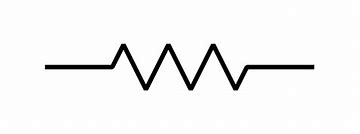
\includegraphics[width=\columnwidth]{resistor}
\caption{Left figure} \label{fig:left}
\end{subfigure}
\hfill
\begin{subfigure}{0.32\columnwidth}
\centering
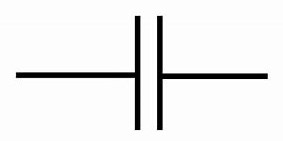
\includegraphics[width=\columnwidth]{capacitor}
\caption{Right figure} \label{fig:right}
\end{subfigure}
\hfill
\begin{subfigure}{0.32\columnwidth}
\centering
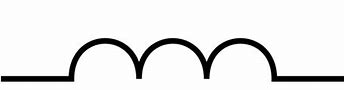
\includegraphics[width=\columnwidth]{indutor}
\caption{Right figure} \label{fig:right}
\end{subfigure}
\caption{Componentes básicos de circuito}
\end{figure}

$$V=RI$$
$$I=C\ \dfrac{dv}{dt}$$
$$V=L\ \dfrac{di}{dt}$$

\section{Conceitos gerais}
Se não tem elétrons livres não há corrente, que é o deslocamento de elétrons. Entretanto, isso só ocorre a 0 Kelvin.
À temperatura ambiente, as ligações covalentes quebram-se devido à energia térmica do meio, formando elétrons livres.

\begin{figure}[H]
\centering
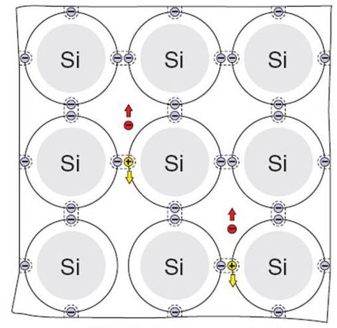
\includegraphics[width=0.75\columnwidth]{silicio}
\caption{Semicondutores: átomos de silício possuem 4 átomos na camada de valência}
\end{figure}


\subsection{Energia de banda proibida}
Quanto maior a energia de banda proibida, mias difícil passar da condição de isolante para condutor.
$ n_i$ é a densidade de elétrons livres.

\begin{figure}[H]
\centering
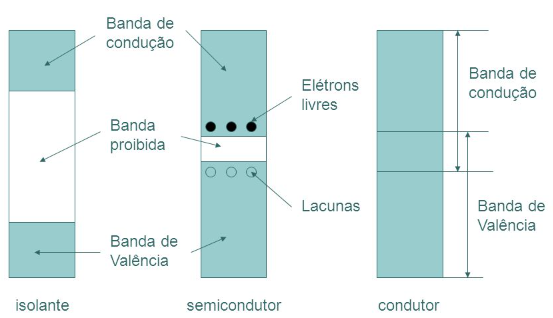
\includegraphics[width=0.9\columnwidth]{banda}
\caption{Semicondutores: estrutura de bandas de energia}
\end{figure}


\begin{equation} \label{eq}
n_i=BT^{\frac{3}{2}} e^{\frac{-Eg}{2KT}}
\end{equation}

$n_i$ é densidade de elétrons do material intrínseco. $K$ é a constante de Boltzmann, $1,38\cdot 10^{-23}$ (J/K) ou $8,62\cdot 10^{5}\  [eV/K]$.

$B$ é uma constante que para o Si varia entre $5,2\cdot 10^15\  [cm^{-3}K^{-3/2}]$ e $7,3\cdot 10^{15}$.\\

$Eg$ é a \emph{Energia de Banda Proibida}:

* Si - $1,2eV$ ou $1,792\cdot 10^{-19}$ [J]\\
\indent*Ge - $0,67$\\


Exercício 001 - Determine a densidade de elétrons livres em um cristal de silício à temperatura de 300K.
Solução:  utilize a equação para cálculo de densidade de elétrons do material intrínseco em \ref{eq}.

%\section{CONCLUSÕES}


%==================================
% REFERÊNCIAS
%==================================
\begin{thebibliography}{9}

%% INTRODUCAO
\bibitem{artigo}	
    L. Chua,
    “Memristor - the missing circuit element”, 
    in \emph{IEEE Transactions on circuit theory}, VOL. CT-18, NO. 5, Setembro 1971.

\end{thebibliography}



\end{multicols}
\end{document}
